\documentclass[11pt]{article}
\usepackage[margin=1in]{geometry}
\usepackage{amsmath,amssymb}
\usepackage{graphicx}
\usepackage[hidelinks]{hyperref}
\usepackage{enumitem}

\setlist[itemize]{leftmargin=1.5em}
\setlist[enumerate]{leftmargin=1.5em}

\newcommand{\Linf}{L_{\infty}}

\title{Literature Status Packet: \(L_2+\Linf\) versus \(L_2\cap\Linf\)}
\author{FA/Banach run \texttt{fa\_banach\_001}}
\date{2026-06-13}

\begin{document}
\maketitle

\section*{Status}

The final problem in Astashkin--Maligranda arXiv:1704.01717 asks whether
\[
  L_2(0,\infty)+L_\infty(0,\infty)
  \quad\text{and}\quad
  L_2(0,\infty)\cap L_\infty(0,\infty)
\]
are isomorphic.  This problem has a later negative answer: Astashkin--Maligranda
arXiv:1804.03469 proves that these two spaces are not isomorphic.

This packet is classified as \texttt{literature\_already\_answered}, not as an
original solution.

\section*{Original Problem Source}

Original source:

\begin{itemize}
\item S. V. Astashkin and L. Maligranda,
\emph{\(L_p+L_\infty\) and \(L_p\cap L_\infty\) are not isomorphic for all
\(1\leq p<\infty\), \(p\neq 2\)}, arXiv:1704.01717;
Proc. Amer. Math. Soc. 146 (2018), no. 5, 2181--2194.
\end{itemize}

The question appears on page 13:

\begin{center}

\includegraphics[width=\textwidth]{figures/open_problem_crop.png}
\end{center}

\section*{Supporting Answer Source}

Supporting source:

\begin{itemize}
\item S. V. Astashkin and L. Maligranda,
\emph{\(L_p+L_q\) and \(L_p\cap L_q\) are not isomorphic for all
\(1\leq p,q\leq\infty\), \(p\neq q\)}, arXiv:1804.03469.
\end{itemize}

The abstract explicitly identifies the \(L_2+\Linf\) case as an answer to a
question in reference [2]:

\begin{center}

\includegraphics[width=\textwidth]{figures/supporting_answer_crop.png}
\end{center}

The supporting paper's Theorem 2 states the exact non-isomorphism:

\begin{center}
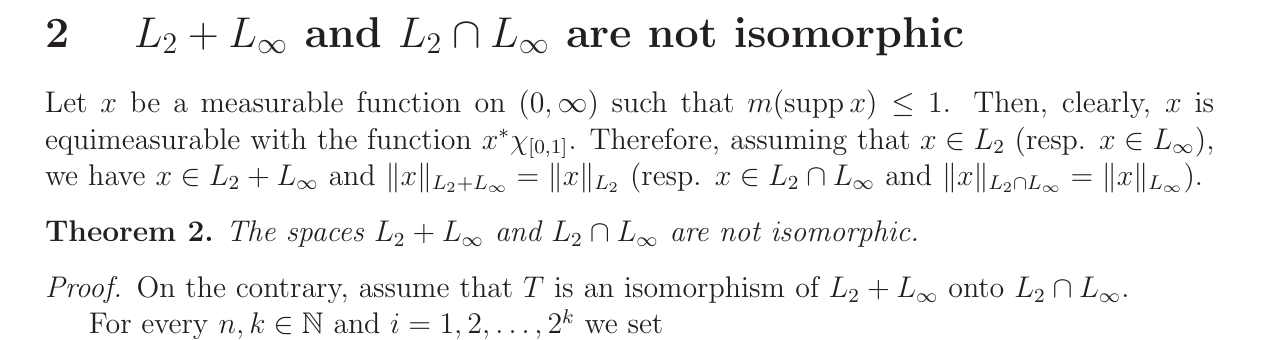
\includegraphics[width=\textwidth]{figures/supporting_theorem_crop.png}
\end{center}

Its reference [2] is the original 2018 PAMS paper:

\begin{center}

\includegraphics[width=\textwidth]{figures/supporting_reference_crop.png}
\end{center}

\section*{Verification Notes}

\begin{itemize}
\item The original paper states the \(L_2+\Linf\) versus \(L_2\cap\Linf\)
question as open in Section 4.
\item The supporting paper is separate and later.  It says that the \(p=2\),
\(q=\infty\) case was the motivation to continue the earlier work.
\item The supporting theorem is stronger than needed: its main theorem gives
non-isomorphism of \(L_p+L_q\) and \(L_p\cap L_q\) for all distinct
\(p,q\in[1,\infty]\).
\end{itemize}

\section*{Search Bounds and Limitations}

Before promotion, the run registry, solution index, attempt index, proof-gap
index, and local parsed source for arXiv:1704.01717 were checked for duplicate
coverage.  Web searches on 2026-06-13 for the original title, arXiv id, and
the \(L_2+\Linf\) / \(L_2\cap\Linf\) phrases located arXiv:1804.03469 as the
direct later answer.

This packet does not address the separate Problem 1 in arXiv:1704.01717 asking
whether \(L_1+\Linf\) is isomorphic to a dual Banach space.

\section*{Human Review Recommendation}

Check the four displayed evidence images: the original question, the supporting
abstract's answer statement, the supporting Theorem 2, and the reference-list
identification of [2].  Together they establish the exact literature-status
transfer.

\end{document}
